\documentclass[a4paper,10pt]{article}
\setlength{\parindent}{0cm}
\usepackage{amsmath, amssymb, amsthm, mathtools,pgfplots}
\usepackage{graphicx,caption}
\usepackage{verbatim}
\usepackage{venndiagram}
\usepackage[cm]{fullpage}
\usepackage{fancyhdr}
\usepackage{tikz}
\usepackage{listings,url,}
\usepackage{color,enumerate,framed}
\usepackage{color,hyperref}
\definecolor{darkblue}{rgb}{0.0,0.0,0.5}
\hypersetup{colorlinks,breaklinks,
            linkcolor=darkblue,urlcolor=darkblue,
            anchorcolor=darkblue,citecolor=darkblue}
\usetikzlibrary{arrows,positioning} 
\usepackage{sectsty}
\allsectionsfont{\centering}
%\usepackage[normalem]{ulem}
%\allsectionsfont{\sffamily}
%\sectionfont{\centering\ulemheading{\uuline}}

%\usepackage{tgadventor}
%\usepackage[nohug]{diagrams}
\usepackage[T1]{fontenc}
%\usepackage{helvet}
%\renewcommand{\familydefault}{\sfdefault}
\usepackage{parskip}
%\usepackage{picins} %for \parpic.
%\newtheorem*{notation}{Notation}
%\newtheorem{example}{Example}[section]
%\newtheorem*{problem}{Problem}
\theoremstyle{definition}
%\newtheorem{theorem}{Theorem}
%\newtheorem*{solution}{Solution}
%\newtheorem*{definition}{Definition}
%\newtheorem{lemma}[theorem]{Lemma}
%\newtheorem{corollary}[theorem]{Corollary}
%\newtheorem{proposition}[theorem]{Proposition}
%\newtheorem*{remark}{Remark}
%\setcounter{section}{1}

\newtheorem{thm}{Theorem}[section]
\newtheorem{lemma}[thm]{Lemma}
\newtheorem{prop}[thm]{Proposition}
\newtheorem{cor}[thm]{Corollary}
\newtheorem{defn}[thm]{Definition}
\newtheorem*{examp}{Example}
\newtheorem{conj}[thm]{Conjecture}
\newtheorem{rmk}[thm]{Remark}
\newtheorem*{nte}{Note}
\newtheorem*{notat}{Notation}

%\diagramstyle[labelstyle=\scriptstyle]

\lstset{frame=tb,
  language=Oz,
  aboveskip=3mm,
  belowskip=3mm,
  showstringspaces=false,
  columns=flexible,
  basicstyle={\small\ttfamily},
  breaklines=true,
  breakatwhitespace=true,
  tabsize=3
}


\pagestyle{fancy}




\fancyhead{}
\renewcommand{\headrulewidth}{0pt}

\lfoot{\color{black!60}{\sffamily Zhangsheng}}
\cfoot{}
\cfoot{\color{black!60}{\sffamily Last modified: \today}}
\rfoot{\color{black!60}{\sffamily\thepage}}



\begin{document}
\begin{flushright}
Zhangsheng Lai
\end{flushright}

This discussion attempts to analyse the cooperation and competition problem using the congestion games approach. The idea was motivated by the opting out example that was discussed in class as it was seen that the structure has some similarities to the problem we are trying to understand here.

\newdimen\R
\R=2cm
\begin{figure}[h]
\centering
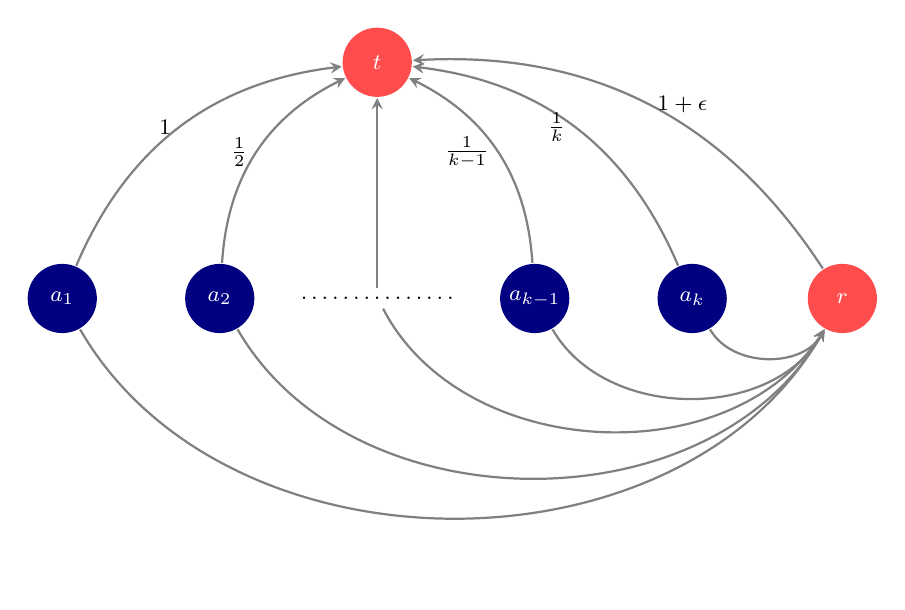
\begin{tikzpicture}[scale=1,draw=black!50,>=stealth,thick]
	\tikzstyle{neuron}=[circle,fill=black!25,
	minimum size=25pt,
	inner sep=0pt
	]
	\tikzstyle{m}=[neuron, fill=blue!50!black];
	\tikzstyle{n}=[neuron, fill=red!70!white];
\footnotesize
\node[n](t) at (0,3){\footnotesize {\color{white}\sffamily $t$}};
%\node[n](r) at (0,-3){\footnotesize {\color{white}\sffamily $r$}};
\node[m](s1) at (-4,0){\footnotesize {\color{white}\sffamily $a_{1}$}};
\node[m](s2) at (-2,0){\footnotesize {\color{white}$a_2$}};
%\node[m](si) at (0,0){\footnotesize {\color{white}$a_i$}};
\node (si) at (0,0){$\ldots \ldots \ldots\ldots \ldots$};
\node[m](sk-1) at (2,0){\footnotesize {\color{white}$a_{k-1}$}};
\node[m](sk) at (4,0){\footnotesize {\color{white}$a_k$}};

\node[n,right=of sk](r) {{\color{white}$r$}}  edge[bend right,->,>=stealth]node[right]{$1+\epsilon$} (t);
%\draw[->,thick,dashed] (r) edge (dummy) edge[thick] (t);



\draw [->] (s1) edge[bend left]node[left]{$1$} (t);
\draw [->,>=stealth] (s2) edge[bend left]node[left]{$\frac{1}{2}$} (t);
\draw [->,>=stealth] (si) edge (t);
\draw [->,>=stealth] (sk-1) edge[bend right]node[left]{$\frac{1}{k-1}$} (t);
\draw [->,>=stealth] (sk) edge[bend right]node[left]{$\frac{1}{k}$} (t);

%\draw[dotted] (s2) edge (si);
%\draw[dotted] (si) edge (sk-1);
\draw [->,>=stealth] (s1) edge[bend right=60](r);
\draw [->,>=stealth] (s2) edge[bend right=60] (r);
\draw [->,>=stealth] (si) edge[bend right=60] (r);
\draw [->,>=stealth] (sk-1) edge[bend right=60] (r);
\draw [->,>=stealth	] (sk) edge[bend right=60] (r);


\end{tikzpicture}
\caption{Opting out problem viewed as a cooperation and competition problem.}
\end{figure}
In a cooperation and competition problem, instead of looking at how much time the agent spends on his own project and how much time on helping other agents, we just consider the nature of the agent; whether the agent is cooperative or competitive. Now we consider a company with $k$ agents and with some measure, we can rank the agents based on their work ability. Here, work ability is with respect to a particular task. For example, if we have two agents, an account and a secretary, the work ability of an account is higher for account work as compared to the secretary and vice versa the work ability of a secretary is higher for secretarial duties. For such a task, we assume that every agent can complete it by himself, however, due to the agent's own work ability for a particular task, the quality of the work produced and the time taken to complete the work varies for different agents. Given the ranking of an agent's work ability for a task $t$ is $i$, the quality of work that they produce is $1/i$. The better your work ability, the better the quality of your work.

Now if we consider scenario with two agents and a particular task $t$ is assigned to one of them, with agent $i$ having rank $i$. If agent 1 was the agent assigned the task, there is no need to find collaborators for the task as the quality of work he is producing is the best. However if the task is assigned to agent 2, then he might want to engage the help of agent 1 to collaborate on that task assigned to him. As such if they collaborate, they would be producing a work of quality $1+\epsilon$ and assuming that they contributed equal effort for the equality of work produced, then there...


a particular task $t$ that is assigned to a particular agent with rank $i$. If $i=1$, the agent does not see the need get collaborators as 




\end{document}